%!TEX program = xelatex
%---------------------------------------------------------------------------%
%-                                                                         -%
%-                           LaTeX Template                                -%
%-                                                                         -%
%---------------------------------------------------------------------------%
%- Copyright (C) Huangrui Mo <huangrui.mo@gmail.com> 
%- This is free software: you can redistribute it and/or modify it
%- under the terms of the GNU General Public License as published by
%- the Free Software Foundation, either version 3 of the License, or
%- (at your option) any later version.
%---------------------------------------------------------------------------%
%->> Document class declaration
%---------------------------------------------------------------------------%
\documentclass[twoside,fontset=none]{Style/ucasthesis}%
%- Multiple optional arguments:
%- [<oneside|twoside|print>]% oneside eprint, twoside eprint, or paper print
%- [fontset=<adobe|none|...>]% specify font set instead of automatic detection
%- [scheme=plain]% thesis writing of international students
%- [draftversion]% show draft version information
%- [standard options for ctex book class: draft|paper size|font size|...]%
%---------------------------------------------------------------------------%
%->> Document settings
%---------------------------------------------------------------------------%
\usepackage[numbers,list,lscape]{Style/artratex}% document settings
%- usage: \usepackage[option1,option2,...,optionN]{artratex}
%- Multiple optional arguments:
%- [bibtex|biber]% set bibliography processor and package
%- [<numbers|super|authoryear|alpha>]% set citation and reference style
%- <numbers>: textual: Jones [1]; parenthetical: [1]
%- <super>: textual: Jones superscript [1]; parenthetical: superscript [1]
%- <authoryear>: textual: Jones (1995); parenthetical: (Jones, 1995)
%- <alpha>: textual: not available; parenthetical: [Jon95]
%- [geometry]% reconfigure page layout via geometry package
%- [lscape]% provide landscape layout environment
%- [xhf]% disable header and footer via fancyhdr package
%- [color]% provide color support via xcolor package
%- [background]% enable page background
%- [tikz]% provide complex diagrams via tikz package
%- [table]% provide complex tables via ctable package
%- [list]% provide enhanced list environments for algorithm and coding
%- [math]% enable some extra math packages
%- [xlink]% disable link colors
\usepackage{Style/artracom}% user defined commands
%---------------------------------------------------------------------------%
%->> Document inclusion
%---------------------------------------------------------------------------%
%\includeonly{Tex/Chap_1,...,Tex/Chap_N}% selected files compilation
%---------------------------------------------------------------------------%
%->> Document content
%---------------------------------------------------------------------------%
%-
%-> Titlepage information
%-
%!TEX root = ../Thesis.tex
%!Mode:: "TeX:UTF-8"
%---------------------------------------------------------------------------%
%->> Titlepage information
%---------------------------------------------------------------------------%
%-
%-> 中文封面信息
%-
\confidential{}% 密级:只有涉密论文才填写
\schoollogo[scale=0.095]{ucas_logo}% 校徽
\title{中国科学院大学学位论文\LaTeX{}模板 {$~^{\pi}\pi^{\pi}$}}% 论文中文题目
\author{张三}% 论文作者
\advisor{李四~~教授~~中国科学院大学工程科学学院\\}% 指导教师:姓名 专业技术职务 工作单位
%\advisor{指导教师一\\指导教师二\\指导教师三}% 多行指导教师示例
\degree{硕士}% 学位:学士、硕士、博士
\degreetype{工学}% 学位类别:理学、工学、工程、医学等
\major{计算机应用技术}% 二级学科专业名称
\institute{中国科学院工程科学学院}% 院系名称
%\institute{中国科学院力学研究所\\流固耦合实验室}% 多行院系名称示例
\date{2023~年~6~月}% 毕业日期:夏季为6月、冬季为12月
%-
%-> 英文封面信息
%-
\TITLE{\LaTeX{} Thesis Template\\ of \\ The University of Chinese Academy of Sciences {$~^{\pi}\pi^{\pi}$}}% 论文英文题目
\AUTHOR{ZHANG San}% 论文作者
\ADVISOR{Supervisor: Professor LI Si}% 指导教师
\DEGREE{Master}% 学位:Bachelor, Master, Doctor, Postdoctor。封面据英文学位名称自动切换,需确保拼写准确
\DEGREETYPE{Science in Engineering}% 学位类别:Philosophy, Natural Science, Engineering, Economics, Agriculture 等
\MAJOR{Computer Applied Technology}% 二级学科专业名称
\INSTITUTE{School of Engineering Science, University of Chinese Academy of Sciences}% 院系名称
\DATE{June, 2014}% 毕业日期:夏季为June、冬季为December
%---------------------------------------------------------------------------%
%
\begin{document}
%-
%-> Frontmatter: title page, abstract, content list, symbol list, preface
%-
\frontmatter% initialize the environment
%!TEX root = ../Thesis.tex
%!Mode:: "TeX:UTF-8"
%---------------------------------------------------------------------------%
%->> Frontmatter
%---------------------------------------------------------------------------%
%-
%-> 生成封面
%-
\maketitle% 生成中文封面
\MAKETITLE% 生成英文封面
%-
%-> 作者声明
%-
\makedeclaration% 生成声明页
%-
%-> 中文摘要
%-
\intobmk\chapter*{摘\quad 要}% 显示在书签但不显示在目录
\setcounter{page}{1}% 开始页码
\pagenumbering{Roman}% 页码符号

本文是中国科学院大学学位论文模板ucasthesis的使用说明文档。主要内容为介绍\LaTeX{}文档类ucasthesis的用法,以及如何使用\LaTeX{}快速高效地撰写学位论文。

中文摘要、英文摘要、目录、论文正文、参考文献、附录、致谢、攻读学位期间发表的学术论文与其他相关学术成果等均须由另页右页(奇数页)开始。

\keywords{中国科学院大学,学位论文,\LaTeX{}模板}% 中文关键词
%-
%-> 英文摘要
%-
\intobmk\chapter*{Abstract}% 显示在书签但不显示在目录

This paper is a help documentation for the \LaTeX{} class \texttt{ucasthesis}, which is a thesis template for the University of Chinese Academy of Sciences. The main content is about how to use the \texttt{ucasthesis}, as well as how to write a thesis efficiently by using \LaTeX{}.

Chinese abstracts, English abstracts, table of contents, the main contents, references, appendix, acknowledgments, author's resume and academic papers published during the degree study and other relevant academic achievements must start with another right page (odd-numbered page).

\KEYWORDS{University of Chinese Academy of Sciences (UCAS), Thesis, \LaTeX{} Template}% 英文关键词

\pagestyle{enfrontmatterstyle}%
\cleardoublepage\pagestyle{frontmatterstyle}%

%---------------------------------------------------------------------------%
% title page, abstract
{% content list region
\linespread{1.2}% local line space
\intobmk*{\cleardoublepage}{\contentsname}% add link to bookmark
\tableofcontents% content catalog
\intobmk*{\cleardoublepage}{\listfigurename}% add link to bookmark
\listoffigures% figure catalog
\intobmk*{\cleardoublepage}{\listtablename}% add link to bookmark
\listoftables% table catalog
}
%!TEX root = ../Thesis.tex
%!Mode:: "TeX:UTF-8"

\intobmk\chapter*{符号列表}% 显示在书签但不显示在目录

\section*{字符}
\nomenclatureitem[\textbf{Unit}]{\textbf{Symbol}}{\textbf{Description}}
\nomenclatureitem[$\Unit{m^{2} \cdot s^{-2} \cdot K^{-1}}$]{$R$}{the gas constant}
\nomenclatureitem[$\Unit{m^{2} \cdot s^{-2} \cdot K^{-1}}$]{$C_v$}{specific heat capacity at constant volume}
\nomenclatureitem[$\Unit{m^{2} \cdot s^{-2} \cdot K^{-1}}$]{$C_p$}{specific heat capacity at constant pressure}
\nomenclatureitem[$\Unit{m^{2} \cdot s^{-2}}$]{$E$}{specific total energy}
\nomenclatureitem[$\Unit{m^{2} \cdot s^{-2}}$]{$e$}{specific internal energy}
\nomenclatureitem[$\Unit{m^{2} \cdot s^{-2}}$]{$h_T$}{specific total enthalpy}
\nomenclatureitem[$\Unit{m^{2} \cdot s^{-2}}$]{$h$}{specific enthalpy}
\nomenclatureitem[$\Unit{kg \cdot m \cdot s^{-3} \cdot K^{-1}}$]{$k$}{thermal conductivity}
\nomenclatureitem[$\Unit{kg \cdot m^{-1} \cdot s^{-2}}$]{$S_{ij}$}{deviatoric stress tensor}
\nomenclatureitem[$\Unit{kg \cdot m^{-1} \cdot s^{-2}}$]{$\tau_{ij}$}{viscous stress tensor}
\nomenclatureitem[$\Unit{1}$]{$\delta_{ij}$}{Kronecker tensor}
\nomenclatureitem[$\Unit{1}$]{$I_{ij}$}{identity tensor}

\section*{算子}
\nomenclatureitem{\textbf{Symbol}}{\textbf{Description}}
\nomenclatureitem{$\Delta$}{difference}
\nomenclatureitem{$\nabla$}{gradient operator}
\nomenclatureitem{$\delta^{\pm}$}{upwind-biased interpolation scheme}

\section*{缩写}
\nomenclatureitem{CFD}{Computational Fluid Dynamics}
\nomenclatureitem{CFL}{Courant-Friedrichs-Lewy}
\nomenclatureitem{EOS}{Equation of State}
\nomenclatureitem{JWL}{Jones-Wilkins-Lee}
\nomenclatureitem{WENO}{Weighted Essentially Non-oscillatory}
\nomenclatureitem{ZND}{Zel'dovich-von Neumann-Doering}

% symbol list, preface content
%-
%-> Mainmatter
%-
\mainmatter% initialize the environment
%---------------------------------------------------------------------------%
%->> Main content
%---------------------------------------------------------------------------%
%!TEX root = ../Thesis.tex
%!Mode:: "TeX:UTF-8"

\chapter{绪论}\label{chap:introduction}

\section{背景}

2022年修订的《中国科学院大学研究生学位论文撰写规范和指导意见》(以下简称《指导意见》)从2023年冬季批次开始实施。为方便各位同学使用,特提供此模板。

您在使用此模板进行学位论文撰写时,只需根据《指导意见》在相应章节填写具体内容即可。

本模板在第2章提供了本模板的使用说明,在第3章中提供了《指导意见》中关于内容和格式的部分要求,请仔细阅读。


\section{系统要求}\label{sec:system}
\begin{table}
    \bicaption{支持的LaTeX编译系统和编辑器}{Supported LaTeX compiler and editor}% caption
    \footnotesize% fontsize
    \setlength{\tabcolsep}{4pt}% column separation
    \renewcommand{\arraystretch}{1.5}% row space 
    \centering
    \begin{tabular}{lcc}
        \hline
        %\multicolumn{num_of_cols_to_merge}{alignment}{contents} \\
        %\cline{i-j}% partial hline from column i to column j
        操作系统 & LaTeX编译系统 & LaTeX文本编辑器\\
        \hline
        Windows & \href{https://www.tug.org/texlive/acquire-netinstall.html}{TexLive Full} 或 \href{https://miktex.org/download}{MiKTex} & \href{http://www.xm1math.net/texmaker/}{Texmaker}\\
        Linux & \href{https://www.tug.org/texlive/acquire-netinstall.html}{TexLive Full} & \href{http://www.xm1math.net/texmaker/}{Texmaker} 或 Vim\\
        MacOS & \href{https://www.tug.org/mactex/}{MacTex Full} & \href{http://www.xm1math.net/texmaker/}{Texmaker} 或 Texshop\\
        Overleaf & XeLaTeX+TexLive2021 & Overleaf \\
        \hline
    \end{tabular}
    \label{tab:compiler}
\end{table}
\href{https://github.com/mohuangrui/ucasthesis}{\texttt{ucasthesis}} 宏包可以在目前主流的 \href{https://en.wikibooks.org/wiki/LaTeX/Introduction}{LaTeX} 编译系统中使用,如TexLive和MiKTeX。因CTex套装已停止维护,\textbf{不再建议使用} (请勿混淆CTex套装与ctex宏包。CTex套装是集成了许多LaTeX组件的LaTeX编译系统。 \href{https://ctan.org/pkg/ctex?lang=en}{ctex} 宏包如同ucasthesis,是LaTeX命令集,其维护状态活跃,并被主流的LaTeX编译系统默认集成,是几乎所有LaTeX中文文档的核心架构)。推荐的 \href{https://en.wikibooks.org/wiki/LaTeX/Installation}{LaTeX编译系统} 和 \href{https://en.wikibooks.org/wiki/LaTeX/Installation}{LaTeX文本编辑器} 为LaTeX编译系统见表~\ref{tab:compiler}。请从各软件官网下载安装程序,勿使用不明程序源。LaTeX编译系统和LaTeX编辑器分别安装成功后,即完成了LaTeX的系统配置,无需其他手动干预和配置。若系统原带有旧版的LaTeX编译系统并想安装新版,请\textbf{先卸载干净旧版再安装新版}。

使用overleaf在线编辑是一种简单有效的方法,对于绝大多数初学者来说,我们推荐使用这种无需进行系统配置的方式。在操作时,只需将压缩包上传至网站即可,无需在本地配置环境,同时支持多人,多地撰写论文。

本模板兼容操作系统:Windows、Linux、MacOS、Overleaf在线编辑器,支持多种LaTeX编译引擎(pdfLaTeX、xeLaTeX、luaLaTeX)。

%!TEX root = ../Thesis.tex
%!Mode:: "TeX:UTF-8"
\chapter{\LaTeX{}使用说明}\label{chap:guide}

本模板基于 \href{https://github.com/mohuangrui/ucasthesis}{ucasthesis} 修改而成。

为方便使用及更好地展示\LaTeX{}排版的优秀特性,ucasthesis的框架和文件体系进行了细致地处理,尽可能地对各个功能和板块进行了模块化和封装,对于初学者来说,众多的文件目录也许一开始让人觉得有些无所适从,但阅读完下面的使用说明后,会发现原来使用思路是简单而清晰的,而且,当对\LaTeX{}有一定的认识和了解后,会发现其相对Word类排版系统极具吸引力的优秀特性。所以,如果是初学者,请不要退缩,请稍加尝试和坚持,以领略到\LaTeX{}的非凡魅力,并可以通过阅读相关资料如\LaTeX{} Wikibook \citep{wikibook2014latex} 来完善自己的使用知识。

\section{先试试效果}

\begin{enumerate}
    \item 安装软件:根据所用操作系统和章节~\ref{sec:system}中的信息安装\LaTeX{}编译环境。
    \item 获取模板:下载 \href{https://github.com/jianxuecn/ucasiiplthesis}{ucasiiplthesis} 模板并解压。ucasiiplthesis模板不仅提供了相应的类文件,同时也提供了包括参考文献等在内的完成学位论文的一切要素,所以,下载时,推荐下载整个ucasiiplthesis文件夹,而不是单独的文档类。
    \item 编译模板:
        \begin{enumerate}
            \item Windows:双击运行artratex.bat脚本。
            \item Linux或MacOS: {\scriptsize \verb|terminal| -> \verb|chmod +x ./artratex.sh| -> \verb|./artratex.sh xa|}
            \item 任意系统:都可使用\LaTeX{}编辑器打开Thesis.tex文件并选择xelatex编译引擎进行编译。
        \end{enumerate}
    \item 错误处理:若编译中遇到了问题,请先查看“常见问题”(章节~\ref{sec:qa})。
\end{enumerate}

编译完成即可获得本PDF说明文档。而这也完成了学习使用ucasthesis撰写论文的一半进程。什么?这就学成一半了,这么简单???,是的,就这么简单!

\section{文档目录简介}

\subsection{Thesis.tex}

Thesis.tex为主文档,其设计和规划了论文的整体框架,通过对其的阅读可以了解整个论文框架的搭建。

\subsection{编译脚本}

\begin{itemize}
    \item Windows:双击Dos脚本artratex.bat可得全编译后的PDF文档,其存在是为了帮助不了解\LaTeX{}编译过程的初学者跨过编译这第一道坎,请勿通过邮件传播和接收此脚本,以防范Dos脚本的潜在风险。
    \item Linux或MacOS:在terminal中运行
        \begin{itemize}
            \item \verb|./artratex.sh xa|:获得全编译后的PDF文档
            \item \verb|./artratex.sh x|:快速编译,不会生成文献引用
        \end{itemize}
\end{itemize}

全编译指运行 \verb|xelatex+bibtex+xelatex+xelatex| 以正确生成所有的引用链接,如目录,参考文献及引用等。在写作过程中若无添加新的引用,则可用快速编译,即只运行一遍\LaTeX{}编译引擎以减少编译时间。

\subsection{Tmp文件夹}

运行编译脚本后,编译所生成的文档皆存于Tmp文件夹内,包括编译得到的PDF文档,其存在是为了保持工作空间的整洁,因为好的心情是很重要的。

\subsection{Style文件夹}

包含ucasthesis文档类的定义文件和配置文件,通过对它们的修改可以实现特定的模版设定。

\begin{enumerate}
    \item ucasthesis.cls:文档类定义文件,论文的最核心的格式即通过它来定义的。
    \item ucasthesis.cfg:文档类配置文件,设定如目录显示为“目~录”而非“目录”。
    \item artratex.sty: 常用宏包及文档设定,如参考文献样式、文献引用样式、页眉页脚设定等。这些功能具有开关选项,常只需在Thesis.tex中进行启用即可,一般无需修改artratex.sty本身。
    \item artracom.sty:自定义命令以及添加宏包的推荐放置位置。
\end{enumerate}

\subsection{Tex文件夹}

文件夹内为论文的所有实体内容,正常情况下,这也是\textbf{使用ucasthesis撰写学位论文时,主要关注和修改的一个位置,注:所有文件都必须采用UTF-8编码,否则编译后将出现乱码文本},详细分类介绍如下:

\begin{itemize}
    \item Frontinfo.tex:为论文中英文封面信息。\textbf{论文封面会根据英文学位名称如Bachelor,Master,Doctor, Postdoctor 自动切换为相应的格式}。
    \item Frontmatter.tex:为论文前言内容如中英文摘要等。
    \item Mainmatter.tex:索引需要出现的Chapter。开始写论文时,可以只索引当前章节,以快速编译查看,当论文完成后,再对所有章节进行索引即可。
    \item Chap{\_}xxx.tex:为论文主体的各章,可根据需要添加和撰写。\textbf{添加新章时,可拷贝一个已有的章文件再重命名,以继承文档的 UTF8 编码}。
    \item Appendix.tex:为附录内容。
    \item Backmatter.tex:为发表文章信息和致谢部分等。
\end{itemize}

\subsection{Img文件夹}

用于放置论文中所需要的图类文件,支持格式有:.jpg, .png, .pdf。其中,\verb|ucas_logo.pdf|为国科大校徽。不建议为各章节图片建子目录,即使图片众多,若命名规则合理,图片查询亦是十分方便。

\subsection{Biblio文件夹}

\begin{enumerate}
    \item ref.bib:参考文献信息库。
\end{enumerate}

\section{数学公式、图表、参考文献等功能}

\subsection{数学公式}

比如Navier-Stokes方程(方程~\eqref{eq:ns}):
\begin{equation} \label{eq:ns}
    %\adddotsbeforeeqnnum%
    \begin{cases}
        \frac{\partial \rho}{\partial t} + \nabla\cdot(\rho\Vector{V}) = 0 \ \mathrm{times\ math\ test: 1,2,3,4,5}, 1,2,3,4,5\\
        \frac{\partial (\rho\Vector{V})}{\partial t} + \nabla\cdot(\rho\Vector{V}\Vector{V}) = \nabla\cdot\Tensor{\sigma} \ \text{times text test: 1,2,3,4,5}\\
        \frac{\partial (\rho E)}{\partial t} + \nabla\cdot(\rho E\Vector{V}) = \nabla\cdot(k\nabla T) + \nabla\cdot(\Tensor{\sigma}\cdot\Vector{V})
    \end{cases}
\end{equation}
\begin{equation}
    %\adddotsbeforeeqnnum%
    \frac{\partial }{\partial t}\int\limits_{\Omega} u \, \mathrm{d}\Omega + \int\limits_{S} \unitVector{n}\cdot(u\Vector{V}) \, \mathrm{d}S = \dot{\phi}
\end{equation}
\[
    \begin{split}
        \mathcal{L} \{f\}(s) &= \int _{0^{-}}^{\infty} f(t) e^{-st} \, \mathrm{d}t, \ 
        \mathscr{L} \{f\}(s) = \int _{0^{-}}^{\infty} f(t) e^{-st} \, \mathrm{d}t\\
        \mathcal{F} {\bigl (} f(x+x_{0}) {\bigr )} &= \mathcal{F} {\bigl (} f(x) {\bigr )} e^{2\pi i\xi x_{0}}, \ 
        \mathscr{F} {\bigl (} f(x+x_{0}) {\bigr )} = \mathscr{F} {\bigl (} f(x) {\bigr )} e^{2\pi i\xi x_{0}}
    \end{split}
\]

数学公式常用命令请见 \href{https://en.wikibooks.org/wiki/LaTeX/Mathematics}{WiKibook Mathematics}。artracom.sty中对一些常用数据类型如矢量矩阵等进行了封装,这样的好处是如有一天需要修改矢量的显示形式,只需单独修改artracom.sty中的矢量定义即可实现全文档的修改。

\subsection{数学环境}

\begin{axiom}
   这是一个公理。 
\end{axiom}
\begin{theorem}
   这是一个定理。 
\end{theorem}
\begin{lemma}
   这是一个引理。 
\end{lemma}
\begin{corollary}
   这是一个推论。 
\end{corollary}
\begin{assertion}
   这是一个断言。 
\end{assertion}
\begin{proposition}
   这是一个命题。 
\end{proposition}
\begin{proof}
    这是一个证明。
\end{proof}
\begin{definition}
    这是一个定义。
\end{definition}
\begin{example}
    这是一个例子。
\end{example}
\begin{remark}
    这是一个注。
\end{remark}

\subsection{表格}

请见表~\ref{tab:sample}。
\begin{table}[!htbp]
    \bicaption{这是一个样表}{This is a sample table}
    \label{tab:sample}
    \centering
    \footnotesize% fontsize
    \setlength{\tabcolsep}{4pt}% column separation
    \renewcommand{\arraystretch}{1.2}%row space 
    \begin{tabular}{lcccccccc}
        \hline
        行号 & \multicolumn{8}{c}{跨多列的标题}\\
        %\cline{2-9}% partial hline from column i to column j
        \hline
        Row 1 & $1$ & $2$ & $3$ & $4$ & $5$ & $6$ & $7$ & $8$\\
        Row 2 & $1$ & $2$ & $3$ & $4$ & $5$ & $6$ & $7$ & $8$\\
        Row 3 & $1$ & $2$ & $3$ & $4$ & $5$ & $6$ & $7$ & $8$\\
        Row 4 & $1$ & $2$ & $3$ & $4$ & $5$ & $6$ & $7$ & $8$\\
        \hline
    \end{tabular}
\end{table}

制图制表的更多范例,请见 \href{https://github.com/mohuangrui/ucasthesis/wiki}{ucasthesis 知识小站} 和 \href{https://en.wikibooks.org/wiki/LaTeX/Tables}{WiKibook Tables}。

\subsection{图片插入}

论文中图片的插入通常分为单图和多图,下面分别加以介绍:

单图插入:假设插入名为\verb|c06h06|(后缀可以为.jpg、.png、.pdf,下同)的图片,其效果如图~\ref{fig:c06h06}。
\begin{figure}[!htbp]
    \centering
    \includegraphics[width=0.40\textwidth]{c06h06}
    \bicaption[Q判据等值面图]{Q判据等值面图,同时测试一下一个很长的标题,比如这真的是一个很长很长很长很长很长很长很长很长的标题。}[Isocontour of Q criteria]{Isocontour of Q criteria, at the same time, this is to test a long title, for instance, this is a really very long very long very long very long very long title.}
    \label{fig:c06h06}
\end{figure}

如果插图的空白区域过大,以图片\verb|c06h06|为例,自动裁剪如图~\ref{fig:c06h06_trim}。
\begin{figure}[!htbp]
    \centering
    %trim option's parameter order: left bottom right top
    \includegraphics[trim = 60mm 80mm 60mm 60mm, clip, width=0.40\textwidth]{c06h06}
    \bicaption{激波圆柱作用}{Shock-cylinder interaction}
    \label{fig:c06h06_trim}
\end{figure}

多图的插入如图~\ref{fig:oaspl},多图应在子图中给文本子标题,主标题尽量简洁,详细说明在正文中给出。子图的引用:图\ref{fig:oaspl_a}。
\begin{figure}[!htbp]
    \centering
    \begin{subfigure}[b]{0.35\textwidth}
      \includegraphics[width=\textwidth]{oaspl_a}
      \caption{子图说明}
      \label{fig:oaspl_a}
    \end{subfigure}%
    ~% add desired spacing
    \begin{subfigure}[b]{0.35\textwidth}
      \includegraphics[width=\textwidth]{oaspl_b}
      \caption{子图说明}
      \label{fig:oaspl_b}
    \end{subfigure}
    \\% line break
    \begin{subfigure}[b]{0.35\textwidth}
      \includegraphics[width=\textwidth]{oaspl_c}
      \caption{子图说明}
      \label{fig:oaspl_c}
    \end{subfigure}%
    ~% add desired spacing
    \begin{subfigure}[b]{0.35\textwidth}
      \includegraphics[width=\textwidth]{oaspl_d}
      \caption{子图说明}
      \label{fig:oaspl_d}
    \end{subfigure}
    \bicaption{总声压级}{OASPL}
    \label{fig:oaspl}
\end{figure}

\subsection{算法}

如见算法~\ref{alg:euclid},详细使用方法请参见文档 \href{https://ctan.org/pkg/algorithmicx?lang=en}{algorithmicx}。

\begin{algorithm}[!htbp]
    \small
    \caption{Euclid's algorithm}\label{alg:euclid}
    \begin{algorithmic}[1]
        \Procedure{Euclid}{$a,b$}\Comment{The g.c.d. of a and b}
        \State $r\gets a\bmod b$
        \While{$r\not=0$}\Comment{We have the answer if r is 0}
        \State $a\gets b$
        \State $b\gets r$
        \State $r\gets a\bmod b$
        \EndWhile\label{euclidendwhile}
        \State \textbf{return} $b$\Comment{The gcd is b}
        \EndProcedure
    \end{algorithmic}
\end{algorithm}

\subsection{参考文献引用}

参考文献引用过程以实例进行介绍,假设需要引用名为"Document Preparation System"的文献,步骤如下:

1)使用Google Scholar搜索Document Preparation System,在目标条目下点击Cite,展开后选择Import into BibTeX打开此文章的BibTeX索引信息,将它们copy添加到ref.bib文件中(此文件位于Biblio文件夹下)。

2)索引第一行 \verb|@article{lamport1986document,|中 \verb|lamport1986document| 即为此文献的label (\textbf{中文文献也必须使用英文label},一般遵照:姓氏拼音+年份+标题第一字拼音的格式),想要在论文中索引此文献,有两种索引类型:

文本类型:\verb|\citet{lamport1986document}|。正如此处所示 \citet{lamport1986document}; 

括号类型:\verb|\citep{lamport1986document}|。正如此处所示 \citep{lamport1986document}。

\textbf{多文献索引用英文逗号隔开}:

\verb|\citep{lamport1986document, chu2004tushu, chen2005zhulu}|。正如此处所示 \citep{lamport1986document, chu2004tushu, chen2005zhulu}

更多例子如:

\citet{walls2013drought} 根据 \citet{betts2005aging} 的研究,首次提出...。其中关于... \citep{walls2013drought, betts2005aging},是当前中国...得到迅速发展的研究领域 \citep{chen1980zhongguo, bravo1990comparative}。引用同一著者在同一年份出版的多篇文献时,在出版年份之后用
英文小写字母区别,如:\citep{yuan2012lana, yuan2012lanb, yuan2012lanc} 和 \citet{yuan2012lana, yuan2012lanb, yuan2012lanc}。同一处引用多篇文献时,按出版年份由近及远依次标注。例如 \citep{chen1980zhongguo, stamerjohanns2009mathml, hls2012jinji, niu2013zonghe}。

使用著者-出版年制(authoryear)式参考文献样式时,中文文献必须在BibTeX索引信息的 \textbf{key} 域(请参考ref.bib文件)填写作者姓名的拼音,才能使得文献列表按照拼音排序。参考文献表中的条目(不排序号),先按语种分类排列,语种顺 序是:中文、日文、英文、俄文、其他文种。然后,中文按汉语拼音字母顺序排列,日文按第一著者的姓氏笔画排序,西文和 俄文按第一著者姓氏首字母顺序排列。如中 \citep{niu2013zonghe}、日 \citep{Bohan1928}、英 \citep{stamerjohanns2009mathml}、俄 \citep{Dubrovin1906}。

如此,即完成了文献的索引,请查看下本文档的参考文献一章,看看是不是就是这么简单呢?是的,就是这么简单!

不同文献样式和引用样式,如著者-出版年制(authoryear)、顺序编码制(numbers)、上标顺序编码制(super)可在Thesis.tex中对artratex.sty调用实现,详见 \href{https://github.com/mohuangrui/ucasthesis/wiki}{ucasthesis 知识小站之文献样式}

%若在上标顺序编码制(super)模式下,希望在特定位置将上标改为嵌入式标,可使用 \citetns{niu2013zonghe,stamerjohanns2009mathml} 和 \citepns{niu2013zonghe,stamerjohanns2009mathml}。

参考文献索引的更多知识,请见 \href{https://en.wikibooks.org/wiki/LaTeX/Bibliography_Management}{WiKibook Bibliography}。\nocite{*}% 使文献列表显示所有参考文献(包括未引用文献)

\section{常见使用问题}\label{sec:qa}

\begin{enumerate}
    \item 模板每次发布前,都已在Windows,Linux,MacOS系统上测试通过。下载模板后,若编译出现错误,则请见 \href{https://github.com/mohuangrui/ucasthesis/wiki}{ucasthesis知识小站} 的 \href{https://github.com/mohuangrui/ucasthesis/wiki/%E7%BC%96%E8%AF%91%E6%8C%87%E5%8D%97}{编译指南}。

    \item 模板文档的编码为UTF-8编码。所有文件都必须采用UTF-8编码,否则编译后生成的文档将出现乱码文本。若出现文本编辑器无法打开文档或打开文档乱码的问题,请检查编辑器对UTF-8编码的支持。如果使用WinEdt作为文本编辑器(\textbf{不推荐使用}),应在其Options -> Preferences -> wrapping选项卡下将两种Wrapping Modes中的内容:
        
        TeX;HTML;ANSI;ASCII|DTX...
        
        修改为:TeX;\textbf{UTF-8|ACP;}HTML;ANSI;ASCII|DTX...
        
        同时,取消Options -> Preferences -> Unicode中的Enable ANSI Format。

    \item 推荐选择xelatex或lualatex编译引擎编译中文文档。编译脚本的默认设定为xelatex编译引擎。你也可以选择不使用脚本编译,如直接使用 \LaTeX{}文本编辑器编译。注:\LaTeX{}文本编辑器编译的默认设定为pdflatex编译引擎,若选择xelatex或lualatex编译引擎,请进入下拉菜单选择。为正确生成引用链接和参考文献,需要进行\textbf{全编译}。

    \item Texmaker使用简介
        \begin{enumerate}
            \footnotesize
            \item 使用 Texmaker “打开 (Open)” Thesis.tex。
            \item 菜单 “选项 (Options)” -> “设置当前文档为主文档 (Define as Master Document)”
            \item 菜单 “自定义 (User)” -> “自定义命令 (User Commands)” -> “编辑自定义命令 (Edit User Commands)” -> 左侧选择 “command 1”,右侧 “菜单项 (Menu Item)” 填入 Auto Build -> 点击下方“向导 (Wizard)” -> “添加 (Add)”: xelatex + bibtex + xelatex + xelatex + pdf viewer -> 点击“完成 (OK)”
            \item 使用 Auto Build 编译带有未生成引用链接的源文件,可以仅使用 xelatex 编译带有已经正确生成引用链接的源文件。
            \item 编译完成,“查看(View)” PDF,在PDF中 “ctrl+click” 可链接到相对应的源文件。
        \end{enumerate}
    
    \item 模版的设计可能地考虑了适应性。致谢等所有条目都是通过最为通用的

        \verb+\chapter{item name}+  and \verb+\section*{item name}+

        来显式实现的 (请观察Backmatter.tex),从而可以随意添加,放置,和修改,如同一般章节。对于图表目录名称则可在ucasthesis.cfg中进行修改。

    \item 设置文档样式: 在artratex.sty中搜索关键字定位相应命令,然后修改
        \begin{enumerate}
            \item 正文行距系数:启用和设置 \verb|\linespread{1.35}|,相当于行距为1.62倍字体高度,大致相当于Word模板所要求的小四号宋体1.25倍行距。
            \item 参考文献行距:修改 \verb|\setlength{\bibsep}{0.0ex}|
            \item 目录显示级数:修改 \verb|\setcounter{tocdepth}{2}|
            \item 文档超链接的颜色及其显示:修改 \verb|\hypersetup|
        \end{enumerate}

    \item 文档内字体切换方法:
        \begin{itemize}
            \item 宋体:国科大论文模板ucasthesis 或 \textrm{国科大论文模板ucasthesis}
            \item 粗宋体:{\bfseries 国科大论文模板ucasthesis} 或 \textbf{国科大论文模板ucasthesis}
            \item 黑体:{\sffamily 国科大论文模板ucasthesis} 或 \textsf{国科大论文模板ucasthesis}
            \item 粗黑体:{\bfseries\sffamily 国科大论文模板ucasthesis} 或 \textsf{\bfseries 国科大论文模板ucasthesis}
            \item 仿宋:{\ttfamily 国科大论文模板ucasthesis} 或 \texttt{国科大论文模板ucasthesis}
            \item 粗仿宋:{\bfseries\ttfamily 国科大论文模板ucasthesis} 或 \texttt{\bfseries 国科大论文模板ucasthesis}
            \item 楷体:{\itshape 国科大论文模板ucasthesis} 或 \textit{国科大论文模板ucasthesis}
            \item 粗楷体:{\bfseries\itshape 国科大论文模板ucasthesis} 或 \textit{\bfseries 国科大论文模板ucasthesis}
        \end{itemize}
\end{enumerate}

%!TEX root = ../Thesis.tex
%!Mode:: "TeX:UTF-8"

\newcommand*{\ltxcmdname}[1]{\texttt{\textbackslash #1}}
\newcommand*{\ltxenvname}[1]{\texttt{#1}}
\newcommand*{\dif}{\mathop{}\!\mathrm{d}}
\newcommand*{\tc}[1]{\multicolumn{1}{c|}{#1}} %单元格居中对齐

\newcommand*{\figref}[1]{图~\ref{#1}~}
\newcommand*{\secref}[1]{~\ref{#1}~节}
\newcommand*{\tabref}[1]{表~\ref{#1}~}
%\newcommand*{\algref}[1]{算法~\ref{#1}~}
\newcommand*{\codref}[1]{程序~\ref{#1}~}
\newcommand*{\thmref}[1]{定理~\ref{#1}~}
\newcommand*{\axmref}[1]{公理~\ref{#1}~}
\newcommand*{\lemref}[1]{引理~\ref{#1}~}
\newcommand*{\prpref}[1]{命题~\ref{#1}~}
\newcommand*{\defref}[1]{定义~\ref{#1}~}

\newcommand*{\ntcite}[1]{~\cite{#1}~}
\newcommand*{\npcite}[1]{\textsuperscript{\cite{#1}}}

\chapter{智能信息处理实验室毕业论文撰写指南}

\section{对基础模板的调整}

\subsection{字体}
在基础模板关于英文字体和数学字体的设置中,若发现系统中存在开源的XITS字体(XITS-Regular.otf,一般会包含在几大主流 \LaTeX{} 发行版中),
则将所有英文字体都设置为XITS,但XITS字体作为英文衬线字体(serif font)和数学字体的一种开源替代品,本身只是一种times字体,
原模板强行将英文非衬线字体(sans-serif font)、等宽(mono)或打字机(typewrite)字体
都设置成XITS这种times字体,这显然不符合英文排版基本规则。而且用times字体排版那些需要使用等宽字体的内容(典型的如计算机代码等)既不美观又不利于阅读。
因此,此处建议对其进行调整。最简单的做法是直接停用XITS字体,将artratex.sty文件中的“XITS-Regular.otf”改成“NoXITS-Regular.otf”,
使得 \LaTeX{} 找不到该文件而使相关设置失效。如果不得不用XITS字体,则至少在artratex.sty文件中将设置英文非衬线字体和等宽字体的部分注释掉。

关于中文编码和字体,最新的\LaTeX{} 发行版(例如TeX Live 2020等)的支持已经非常完善,但是建议编译时使用 \XeLaTeX{} (\texttt{xelatex})作为编译引擎,
因为 \XeLaTeX{} 对中文编码、字体及中英文混排的支持要比 pdfLaTeX 好太多。
另外需要注意的一点是,强烈建议在所使用的文本编辑工具中将文字编码设置为UTF-8(在Sublime Text 3和TeXstudio中均为默认编码格式),以免不必要的麻烦。

对于中文字体,基础模版已经预设好了大部分格式排版所对应的中文字体,例如章节标题为黑体、正文为宋体,配合英文的\textbf{加粗Text}使用宋体伪粗体、
\textit{斜体Text}使用楷体、\texttt{等宽Text}使用仿宋体等。基础模板使用“伪粗体(\texttt{AutoFakeBold})”的方式定义中文宋体和黑体的粗体字型,
这种方式本质上就是将文字横向以微小位移重复显示多次而呈现出加粗效果,即使在计算机中文字体设计很不规范、缺少对应变化字型的年代,
这也是一种不被推荐的折衷方案,不仅效果差强人意,而且会对生成的pdf文件中的文字拷贝造成困扰。
因此,建议使用比较新的中文开源字体:由Adobe和Google联合开发的\href{https://github.com/adobe-fonts}{思源字体}
(加载文档类\texttt{ucasthesis}时加上参数“\texttt{fontset=none}”)。即使不使用这种方式,也应修改字体配置,去掉\texttt{AutoFakeBold}选项,
而代之以其他替代字体(例如用Microsoft Office软件一般都会捆绑安装的“华文中宋”字体作为宋体的粗体)。

另外,修改后的模版为“\texttt{fontset=none}”选项补充定义了4种常用中文字体,方便撰写正文时快速切换字体,
分别是:{\songti 宋体}、{\heiti 黑体}、{\kaishu 楷书}、{\fangsong 仿宋}。

关于在 \LaTeX{} 中使用中英文字体的基础常识及相关设置方法可参考:\href{https://stone-zeng.github.io/2018-08-08-use-opentype-fonts/}{在 \LaTeX{} 中使用 OpenType 字体}。

\section{撰写样例}\label{sec:samples}

\subsection{列表}
\LaTeX 用于列表的环境有三种:\texttt{itemize}、\texttt{enumerate}和\texttt{description}。

无序列举:
\begin{itemize}
	\item 列举项
	\item 列举项
\end{itemize}

带序号列举:
\begin{enumerate}
	\item 列举项
	\item 列举项
\end{enumerate}

带序号列举可以设定序号格式:
\begin{enumerate}[1).]
	\item 列举项
	\item 列举项
\end{enumerate}

带标签的列举,适用于名词定义:
\begin{description}
	\item[名词1] 解释1
	\item[Name2] Description2
\end{description}

列表环境可以相互嵌套,起始编号可以用 \ltxcmdname{setcounter} 命令改变:
\begin{enumerate}
    %用\setcounter改变起始编号,注意:counter从0起计数,显示的序号为当前counter的值加1
    %所以要设置序号从n开始的话,调用\setcounter{enumi}{n-1}
    \setcounter{enumi}{3}
	\item 列举项
    \begin{itemize}
    	\item 列举项
    	\item 列举项
    \end{itemize}
	\item 列举项
	\begin{enumerate}
    	\item 列举项
    	\item 列举项
	\end{enumerate}
\end{enumerate}


\subsection{数学公式}
段落内的数学公式,有三种输入方式:$E=mc^2$、\(\frac{1}{2}\sqrt{b^2-4ac}\)、\begin{math}\mathbf{n}=[x, y, z]^T\end{math}。

段落间的数学公式也有对应的三种输入方式:
% (1)
$$A=\int_0^1 \frac{\ln{x}}{x}\dif x$$
% (2)
\[
A=\int_0^1 \frac{\ln{x}}{x}\dif x
\]
% (3)
\begin{displaymath}
A=\int_0^1 \frac{\ln{x}}{x}\dif x
\end{displaymath}

带编号的数学公式:
\begin{equation}\label{eq:samples:one}
A=\int_0^1 \frac{\ln{x}}{x}\dif x
\end{equation}

带编号的数学公式组(注意利用列分隔符“\texttt{\&}”对齐):
\begin{align}
{\cal M}ˆ2(\hat{\theta},\theta) &= E[(\hat{\theta} - \theta)ˆ2] \\
{\cal M}ˆ2(\hat{\theta},\theta) &= \textrm{var}ˆ2(\hat{\theta}) + {\cal B}ˆ2(\hat{\theta})
\end{align}

\textbf{特别注意:}此处应避免使用 \ltxenvname{eqnarray} 环境,因为此环境存在很多问题,且与\ltxenvname{amsmath}宏包风格不统一,
具体问题请参考这篇文章“\href{https://tug.org/pracjourn/2006-4/madsen/madsen.pdf}{Avoid eqnarray!}”。

跨行长公式(注意利用“\texttt{\&}”对齐):
\begin{equation}
\begin{split}
a& =b+c-d\\
 & \quad +e-f\\
 & =g+h\\
 & =i
\end{split}
\end{equation}

带子编号的数学公式组:
\begin{subequations}\label{eq:samples:grp}
\begin{align}
a&=b+c\label{eq:samples:grp:a}\\
d&=e+f+g\label{eq:samples:grp:b}\\
h&=i+j\label{eq:samples:grp:c}
\end{align}
\end{subequations}

大型分式:
\begin{equation}
\Re{z} =\frac{n\pi \dfrac{\theta +\psi}{2}}{
        \left(\dfrac{\theta +\psi}{2}\right)^2 + \left( \dfrac{1}{2}
        \log \left\lvert\dfrac{B}{A}\right\rvert\right)^2}.
\end{equation}

带条件赋值:
\begin{equation}
z = \left\{
\begin{array}{ll}
1 & (x>0)\\
0 & (x<0)
\end{array}
\right.
\end{equation}

矩阵的输入用 \texttt{matrix} 环境,以“\texttt{\&}”分列、以“\ltxcmdname{\textbackslash}”或“\ltxcmdname{cr}”分行,下面是一个例子:
\begin{equation}
\left(
  \begin{matrix}
    K_{11} &K_{12} &K_{13} &\ldots &K_{1n}\\
    K_{21} &K_{22} &K_{23} &\ldots &K_{2n}\\
    K_{31} &K_{32} &K_{33} &\ldots &K_{3n}\\
    \vdots &\vdots &\vdots &\ddots &\vdots\\
    K_{n1} &K_{n2} &K_{n3} &\ldots &K_{nn}
  \end{matrix}
\right) \left(
  \begin{matrix}
     D_{1}\\ D_{2}\\ D_{3}\\ \vdots\\ D_{n}
  \end{matrix}
\right) = \left(
  \begin{matrix}
    F_{1}\\ F_{2}\\ F_{3}\\ \vdots\\ F_{n}
  \end{matrix}
\right)
\end{equation}

正文中对公式的引用:公式~\eqref{eq:samples:one}。

\subsection{插图}
为了能得到较好的排版效果,又不必做调整图形位置的乏味工作,\LaTeX 提供了一个浮动图形机制来自动将图形放置到合适的位置。为了使这一机制发挥最大效力,在写作时需注意以下几点:
\begin{enumerate}
	\item \textbf{不要使用依赖于图形放置位置的文本}:使用如“\emph{这幅图…}”或“\emph{下图…}”等短语要求所指图形需在固定位置,
	      而像“{\kaishu 图1.1…}”这样的短语则允许图形出现在任意位置,而且配合\LaTeX 提供的强大的交叉引用功能,
	      完全可以自动生成插图编号并建立超链接。
	\item \textbf{放轻松}:一些刚开始使用\LaTeX 的作者发现图形没有十分准确地出现在他们所想要的位置,往往会着急,并对其进行手工干预,
	      这其实完全没有必要,图形的放置是\LaTeX 的工作,最好放轻松一些,到所有内容都撰写校对完成,最后再对插图位置作必要微调。
	      如果你的论文结构合理,正文内容完整充实,此时你会发现插图都已在该在的位置上,没有调整的必要了。
\end{enumerate}

插图一般被放置在\ltxenvname{figure}环境中,\figref{fig:samples:coordinateaxis}是一个单幅插图的例子。\ltxenvname{figure}环境有一个可选参数允许用户指示图形有可能被放置的位置(实际上所有浮动对象环境均有类似的参数设置,例如\secref{sec:tab}要讲的表格环境),这一选项参数可以是下列字母的任意组合(缺省为\texttt{[tbp]}):
\begin{description}
	\item[\texttt{h}(当前位置)] 将插图放置在正文文本中figure环境出现的地方,如果当前页所剩空间不够,这一参数将不起作用;
	\item[\texttt{t}(顶部)] 将插图放置在页面顶部;
	\item[\texttt{b}(底部)] 将插图放置在页面底部;
	\item[\texttt{p}(浮动页)] 将插图放置在只允许有浮动对象的页面上
\end{description}

通常给出的参数越多,\LaTeX 的排版效果越好,例如\texttt{[htbp]}、\texttt{[tbp]}、\texttt{[htp]}、\texttt{[tp]}等组合的效果都不错。另外,在这些位置参数前面加上一个惊叹号(例如\texttt{[!ht]})会使\LaTeX 忽略应用于文本页的审美条件,试图用最严格的标准来放置浮动图形。

\figref{fig:samples:coordinateaxis}是单幅插图的例子。

%% 单幅插图
\begin{figure}[htbp]
%%图形居中放置
\centering
%%插入图形文件
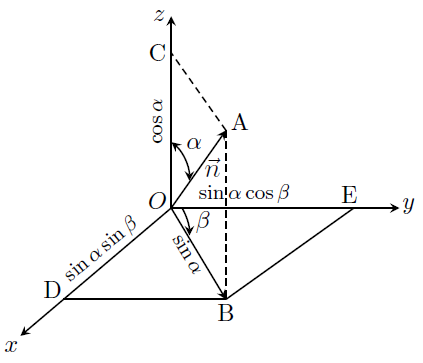
\includegraphics[width=0.45\textwidth]{coordinateaxis}
%                         ^                 ^
%                插图宽度(相对于文本宽)  插图文件名(忽略扩展名)
%% 插图标题(\label 用于设置建立交叉引用的标签名)
\caption{平面的倾角、倾向及其法向矢量}\label{fig:samples:coordinateaxis}
\end{figure}

\figref{fig:samples:blcfy}是包含子图的例子,在\texttt{figure}环境中嵌套\texttt{subfigure}环境即可,参数格式类似,唯一不同的是\texttt{subfigure}不是一个浮动对象(被限制在\texttt{figure}中),因此其位置参数是指子图对齐的方式:\texttt{b}表示底部对齐,\texttt{t}表示顶部对齐。子图间可以用“\ltxcmdname{\textbackslash}”换行。

%% 包含子图的插图
\begin{figure}[htbp]
\def\figwidth{\columnwidth}
  \centering
    \begin{subfigure}[b]{0.5\figwidth} %子图宽度(用相对于整个figure的比例指定)
      \centering
      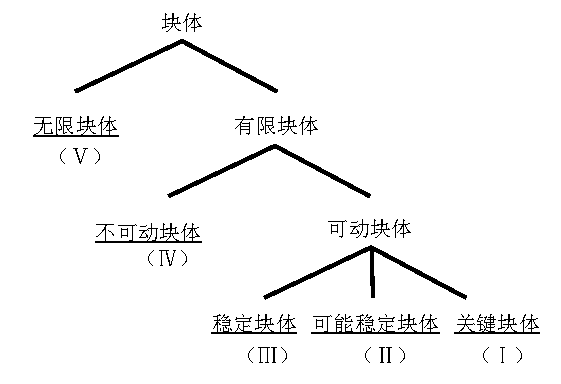
\includegraphics[width=\textwidth]{blockclassify}
      \caption{块体类型}\label{fig:samples:blockclassify}
    \end{subfigure} %此处可以用“\\”换行
    \begin{subfigure}[b]{0.36\figwidth}
      \centering
      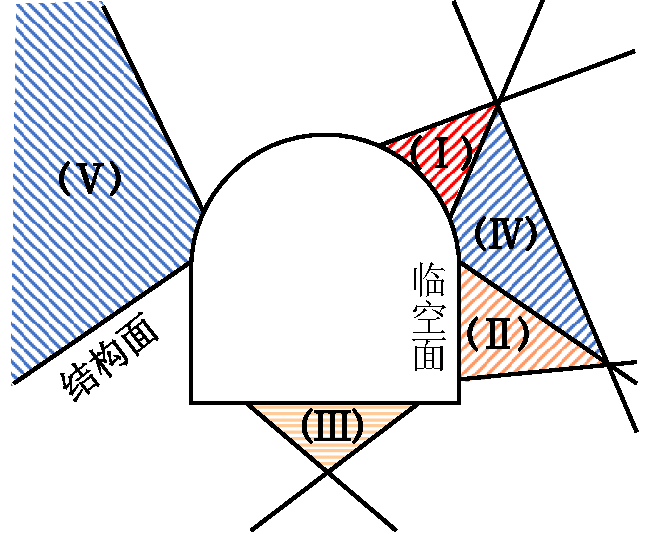
\includegraphics[width=\textwidth]{blockclassify1}
      \caption{平面示意图}\label{fig:samples:blockclassify1}
    \end{subfigure}
  \caption{块体分类}\label{fig:samples:blcfy}
\end{figure}

特别注意,模版支持多种常用插图文件格式,比如\texttt{pdf}、\texttt{png}、\texttt{jpg}、\texttt{tif}等,在用\ltxcmdname{includegraphics}命令引入插图文件时,文件名可以不包含扩展名,\LaTeX 会自行匹配,这样做的好处是当你用另一种更好的文件格式提供同一幅插图时(比如用效果更好的矢量图格式\texttt{pdf}代替原来不够清晰的\texttt{jpg}文件),直接替换插图文件即可,正文中不需要做任何更改。

\subsection{表格}\label{sec:tab}
表格和插图一样,建议使用浮动对象,即将表格放在浮动对象环境\texttt{table}中,例如\tabref{tab:samples:normal}。但是也有一些例外,例如跨页的长表格\texttt{longtable}(\tabref{tab:samples:longtable}),由于不受页面长度限制,所以不必放在浮动对象中,放进去反而会出错。

%% 普通表格
\begin{table}[htbp]
\caption{普通表格示例}\label{tab:samples:normal}
\centering
\begin{tabular}{|>{\tt}c|>{\kaishu}l|>{\tt}l|>{\kaishu}l|}
\hline
  \heiti 变量名 & \tc{\heiti 含义}    & \tc{\heiti 类型} & \tc{\heiti 备注} \\ \hline
  id           & 唯一标识符           & int             & 必须有            \\ \hline
  name         & 名称                & string          &                  \\ \hline
  abbrName     & 名称简写             & string          &                  \\
\hline
\end{tabular}
\end{table}

表格内容的输入则要比插图复杂一些,一般放在\texttt{tabular}环境中,也有的直接放在对应表格环境中(如\texttt{longtable}),列选项在表格环境参数重设置,不同的表格环境其内容大同小异。表格正文内容则一致以“\texttt{\&}”分列、以“\ltxcmdname{\textbackslash}”或“\ltxcmdname{tabularnewline}”断行。表格环境列布局的参数设置比较灵活,可以设定每一列的对齐方式(\texttt{l}、\texttt{r}或\texttt{c},有几个就有几列)、字体(放在“\texttt{>}”后的大括号内)、是否加列间线(“\texttt{|}”)等(详细说明可参考\tabref{tab:samples:longtable})。

此外,还可以使用 \ltxcmdname{multirow}、\ltxcmdname{multicolumn}等命令合并单元格,例如\tabref{tab:samples:threepart}。
\begin{enumerate}
	\item 多行单元格:\ltxcmdname{multirow\{nrows\}[bigstructs]\{width\}[fixup]\{text\}}。其中:\texttt{nrows}设定所占用的行数;\texttt{bigstructs}为可选项,主要是在使用了 bigstruct 宏包时使用;\texttt{width}设定该栏文本的宽度,如果想让 LaTeX 自行决定文本的宽度,则用 * 即可;\texttt{fixup}为可选项,主要用来调整文本的垂直位置;\texttt{text}为所要排版的文本,可用“\ltxcmdname{\textbackslash}”来强制换行。
    \item 多列单元格:\ltxcmdname{multicolumn\{ncols\}\{align\}\{text\}}。其中:\texttt{ncols}设定所占用的列数;\texttt{align}是列选项参数,类似于\texttt{tabular}环境参数,如“\texttt{|c|}”;\texttt{text}为所要排版的文本。
\end{enumerate}

此外,\tabref{tab:samples:threepart}也使用了一个特殊的表格环境\texttt{threeparttable}来生成三线表,此环境主要用处是提供了在表格内加脚注的功能,同时也预定义了一些画各种粗细线条的命令,用于生成不同粗细的表格横线。

%% 三线表及不规则单元格示例
%   (1) 跨行混排
%       \multirow{nrows}[bigstructs]{width}[fixup]{text}
%        nrows       设定所占用的行数。
%        bigstructs  此为可选项,主要是在你使用了 bigstruct 宏包时使用。
%        width       设定该栏文本的宽度。如果想让 LaTeX 自行决定文本的宽度,则用 * 即可。
%        fixup       此为可选项,主要用来调整文本的垂直位置。
%        text        所要排版的文本。可用 \\ 来强迫换行。
%   (2) 跨列混排
%       \multicolumn{ncols}{align}{text}
%        ncols  设定所占用的列数。
%        align  列选项参数,类似于tabular环境参数,如“|c|”。
%        text   所要排版的文本。
\begin{table}[htbp]
\centering
  \begin{threeparttable}
    \newcommand{\chengs}{\ensuremath{\times}}
    \newcommand{\cheng}{\ensuremath{\!\times\!}}
    \caption{三线表及不规则单元格示例}\label{tab:samples:threepart}
    \begin{tabular}{cccc} %指定列数以及每列文字对齐方式:l 左对齐、r 右对齐、c 居中
      \toprule
  \multirow{2}{*}{策略}   & \multirow{2}{*}{尺寸参数}             & \multicolumn{2}{c}{数据量}    \tabularnewline \cmidrule{3-4}
                         &                                      & 数据块数\tnote{a} & 读取像素数\tnote{b} \tabularnewline \midrule
  \multirow{2}{*}{等分}   & $48\chengs 48\chengs 48$             & 2058             & 227598336 \tabularnewline \cmidrule{2-4} %从第2列到第4列画横线
                         & $128\chengs 128\chengs 128$          & 155              & 325058560 \tabularnewline \midrule
  \multirow{2}{*}{自适应} & $[16,64]\cheng[16,64]\cheng[16,64]$  & 1100             & 211624837  \tabularnewline \cmidrule{2-4}
                         & $[16,250]\cheng[16,64]\cheng[16,32]$ & 748              & 219153002  \tabularnewline %“\tabularnewline”相当于“\\”
      \bottomrule
    \end{tabular}
    \begin{tablenotes}\small
      \item[a] 每块数据包括边界
      \item[b] 第二个脚注
    \end{tablenotes}
  \end{threeparttable}
\end{table}

\texttt{longtable}环境用于排版跨页长表,与普通表格不太一样,不能当做浮动对象,当它附近有较多浮动表格对象时有可能导致表格出现的顺序和生成的编号顺序不一致,因此如无必要,建议尽量少用跨页长表,过长的表可以作适当拆分。

%% 跨页长表
\begin{longtable}{|>{\tt}c|>{\kaishu}m{10cm}|}
  \caption{跨页长表示例及表格列选项参数说明} \label{tab:samples:longtable}\\
    \hline \heiti 选项参数 & \tc{\heiti 说明} \\ \endfirsthead %第一页上的表头
  \caption{跨页长表示例及表格列选项参数说明(续)} \\
    \hline \heiti 选项参数 & \tc{\heiti 说明} \\ \endhead %出现在续页上的表头
    \hline         l      & 该列单元格内容左对齐 \\
    \hline         c      & 该列单元格内容居中 \\
    \hline         r      & 该列单元格内容右对齐 \\
    \hline     p\{width\} & 将内容放进一个宽为\texttt{width}的段落盒,等价于\ltxcmdname{parbox[t]\{width\}} \\
    \hline     @\{decl.\} & 删除两边列之间的空白,插入指定的文本,即大括号间的内容\texttt{decl.} \\
    \hline     m\{width\} & 指定列宽为\texttt{width},超出宽度的文字将自动换行,作用接近\ltxcmdname{parbox\{width\}} \\
    \hline     b\{width\} & 相当于\ltxcmdname{parbox[b]\{width\}} \\
    \hline     >\{decl.\} & 可在每个列选项字母之前使用,将大括号间的内容(\texttt{decl.})插入到该列每个单元格内容之前,可以用它来控制每一列的文本格式 \\
    \hline     <\{decl.\} & 可在每个列选项字母之后使用,将大括号间的内容(\texttt{decl.})插入到该列每个单元格内容之后,配合“\texttt{>}”使用可方便地将该列每个单元格放置在一个环境中,比如数学环境 \\
    \hline          |     & 插入一条竖线 \\
    \hline     !\{decl.\} & 与\texttt{|}类似,只不过插入的不是竖线而是大括号间的内容(\texttt{decl.})  \\
    \hline
\end{longtable}

\begin{landscape}% 横排页环境
\pagestyle{lscape}% 横排页眉页脚样式
\begin{longtable}{|>{\tt}c|>{\kaishu}m{10cm}|}
  \bicaption[跨页长表示例]{跨页长表示例及表格列选项参数说明}{Sample for landscape-oriented table over multiple pages and description for the the parameters.} \label{tab:samples:landscapelongtable}\\
    \hline \heiti 选项参数 & \tc{\heiti 说明} \\ \endfirsthead %第一页上的表头
    \multicolumn{2}{c}{\bfseries\small \tablename\ \thetable\ {续表。}} \\
  %\caption{跨页长表示例及表格列选项参数说明(续表)} \\
    \hline \heiti 选项参数 & \tc{\heiti 说明} \\ \endhead %出现在续页上的表头
    \hline \multicolumn{2}{r}{\textit{续表见下页}}\\ \endfoot %续表脚注
    \endlastfoot %最后一页脚注
    \hline         l      & 该列单元格内容左对齐 \\
    \hline         c      & 该列单元格内容居中 \\
    \hline         r      & 该列单元格内容右对齐 \\
    \hline     p\{width\} & 将内容放进一个宽为\texttt{width}的段落盒,等价于\ltxcmdname{parbox[t]\{width\}} \\
    \hline     @\{decl.\} & 删除两边列之间的空白,插入指定的文本,即大括号间的内容\texttt{decl.} \\
    \hline     m\{width\} & 指定列宽为\texttt{width},超出宽度的文字将自动换行,作用接近\ltxcmdname{parbox\{width\}} \\
    \hline     b\{width\} & 相当于\ltxcmdname{parbox[b]\{width\}} \\
    \hline     >\{decl.\} & 可在每个列选项字母之前使用,将大括号间的内容(\texttt{decl.})插入到该列每个单元格内容之前,可以用它来控制每一列的文本格式 \\
    \hline     <\{decl.\} & 可在每个列选项字母之后使用,将大括号间的内容(\texttt{decl.})插入到该列每个单元格内容之后,配合“\texttt{>}”使用可方便地将该列每个单元格放置在一个环境中,比如数学环境 \\
    \hline          |     & 插入一条竖线 \\
    \hline     !\{decl.\} & 与\texttt{|}类似,只不过插入的不是竖线而是大括号间的内容(\texttt{decl.})  \\
    \hline
\end{longtable}
\end{landscape}

\subsection{计算机程序}
计算机源程序可以用 \texttt{lstlisting} 环境排版,代码可直接拷贝进去,除语法高亮外基本原样输出。下面是一个简单的例子:
\begin{lstlisting}
  int PacketQueue::put(AVPacket *pkt) {
      int ret;    
      this->mutex->lock();
      ret = put_private(pkt);
      this->mutex->unlock();    
      if (pkt != &this->flush_pkt && ret < 0) av_packet_unref(pkt);    
      return ret;
  }
\end{lstlisting}

本模版预设按C++语法进行排版及关键字高亮显示,可以用环境参数中切换语言并作其他更细致的设定,例如 \texttt{[language=Pascal]} 将当前 \texttt{lstlisting} 环境切换为 Pascal 语言。同时,页可以通过参数设置将其变为浮动对象:\texttt{[float,caption=A floating example]},如 \codref{lst:samples:pas} 所示。更详细的用法可参考 \texttt{listings} 宏包的说明文档(\texttt{listings.pdf})。
\begin{lstlisting}[float, language=Pascal, caption={浮动代码块}, label={lst:samples:pas}]
  var i:integer;
  var x:integer;
  for i:=maxint to 0 do
  begin
    if (i<=0) then x := 1;
    if (i>0) then x := 0;
  end;
\end{lstlisting}

\subsection{定理}
定理,包括命题、引理、推论等的排版使用 \texttt{theorem}、\texttt{lemma}、\texttt{proposition} 等环境,每个定理可用可选参数指定一个别名。定理的证明放在 \texttt{proof} 环境中,证明结束标志为 \ltxcmdname{qedhere}。

定理示例:
\begin{theorem}[有限性定理] \label{thm:samples:t}
块体为有限的充分必要条件是节理锥(JP)与开挖锥(EP)的交集为空集。
\end{theorem}

公理示例:
\begin{axiom} \label{thm:samples:a}
平面上两点确定一条直线。
\end{axiom}

引理示例:
\begin{lemma} \label{thm:samples:l}
块体为有限的充分必要条件是节理锥(JP)与开挖锥(EP)的交集为空集。
\end{lemma}

命题及证明示例:
\newcommand{\sNP}{\ensuremath{\mathcal{NP}}}
\newcommand{\tNP}{\sNP\ }
\newcommand{\tNPC}{\mbox{\ensuremath{\mathcal{NP}\text{-完全}}}}
\begin{proposition} \label{thm:samples:p}
若有向图的哈密尔顿环路问题是~\tNPC 问题,则无向图的哈密尔顿环路问题也是~\tNPC 问题。
\end{proposition}

\begin{proof}
    显然,无向哈密尔顿环路问题属于~\tNP 问题,因此只要证明有向图的哈密尔顿环路问题可多项式规约到无向图的
    哈密尔顿环路问题~(已知有向图的哈密尔顿问题是~\tNPC 问题)。

    令~$G=(V,E)$ 是包含~$n$ 个顶点的有向图,现将其转换到无向图~$G'=(V',E')$:对每个~$v\in V$,
    $V'$ 中包含~$3$ 个顶点~$v^1,v^2,v^3$ 与之对应,$E'$ 中包含两条无向边~$v^1v^2,v^2v^3$ 与之对应,
    对~$E$ 中的每条边~$vw$,$E'$ 中包含无向边~$v^3w^1$ 与之对应,显然,该转换所需时间以多项式为界,
    若~$|V|=n,|E|=m$ 则~$|V'|=3n,|E'|=2n+m$。

    若~$G$ 中有一条有向哈密尔顿环路~$v_1,\cdots,v_n$,则~$v_1^1,v_1^2,v_1^3,v_2^1,v_2^2,v_2^3,\cdots,$ $v_n^1,v_n^2,v_n^3$ 是~$G'$ 中
    的一条~(无向) 哈密尔顿环路;另一方面,若~$G'$ 中存在一条哈密尔顿环路,由于对每组顶点~$v^1,v^2,v^3$,$v^2$ 只与~$v^1$ 和~$v^3$ 相连,
    因此在环路上必按~$v^1,v^2,v^3$ 或~$v^3,v^2,v^1$ 的顺序访问这三个顶点,而~$G'$ 中的其他边仅连接上标为~$1$ 和~$3$ 的顶点,
    因此该环路上所有的三顶点组要么都按~$1,2,3$ 的顺序排列,要么都按~$3,2,1$ 的顺序排列,
    不妨设该环路为~$v_{i_1}^1,v_{i_1}^2,v_{i_1}^3,\cdots,v_{i_n}^1,v_{i_n}^2,v_{i_n}^3$,则~$v_{i_1},\cdots,v_{i_n}$ 是~$G$ 中的一条
    有向哈密尔顿环路。所以~$G$ 包含有向哈密尔顿环路当且仅当~$G'$ 包含无向哈密尔顿环路。\qedhere
\end{proof}

定义示例:
\begin{definition}[复流形] \label{thm:samples:d}
复流形$M$是一个可微流形,它容许一个开覆盖$\{U_{\alpha}\}$和坐标映射$\varphi_{\alpha}:U_{\alpha}\rightarrow \mathbb{C}^n$ 使得对所有的$\alpha, \beta, \varphi_{\alpha}\circ \varphi_{\beta}^{-1}$在$\varphi_{\beta}(U_{\alpha}\cap U_{\beta})\subset \mathbb{C}^n$是全纯的。
\end{definition}

\subsection{交叉引用}
理论上在文档的任何位置都可以设置交叉引用点,常用的有:特定章节、图、表、公式等。为被引用对象建立交叉引用点的方法是在相应位置使用 \ltxcmdname{label}命令设置一个标签,在需要引用的地方用 \ltxcmdname{ref} 命令建立引用链接,其参数就是前面所设置的标签名称。例如:参见 \ref{sec:samples} 节。由于引用链接只输出\LaTeX 为标签自动生成的编号,所以一般要在 \ltxcmdname{ref} 命令的前后配上相应文字,如“图”、“表”、“公式”等。为省去此琐碎环节,本模版预定义了一些固定的引用模式供大家使用,如:章节引用\secref{sec:samples}、插图引用\figref{fig:samples:blcfy}、表格引用\tabref{tab:samples:normal}、算法引用\algref{alg:euclid}、代码引用\codref{lst:samples:pas}、定理引用\thmref{thm:samples:t}、公理引用\axmref{thm:samples:a}、引理引用\lemref{thm:samples:l}、命题引用\prpref{thm:samples:p}、定义引用\defref{thm:samples:d}等。

另外,还可以使用 \ltxcmdname{pageref}引用对象所在页码,例如:\figref{fig:samples:blcfy}在第 \pageref{fig:samples:blcfy} 页。

页面内的脚注用 \ltxcmdname{footnote}命令添加,例如:此处\footnote{脚注内容。}有脚注。

\subsection{文献引用}\label{sec:samples:cite}
模板提供了一组源自\texttt{natbib}包的引用命令用于不同风格的引用习惯:
\begin{center}
%\linespread{0.5}
%\renewcommand{\arraystretch}{1.0}
\begin{tabular}{lcl}
\verb|\citet{wikibook2014latex}| & $\Rightarrow$ & \citet{wikibook2014latex} \\
\verb|\citet[第2章]{wikibook2014latex}| & $\Rightarrow$ & \citet[第2章]{wikibook2014latex} \\
\verb|\citep{wikibook2014latex}| & $\Rightarrow$ & \citep{wikibook2014latex} \\
\verb|\citep[第2章]{wikibook2014latex}| & $\Rightarrow$ & \citep[第2章]{wikibook2014latex} \\
\verb|\citep[see][第2章]{wikibook2014latex}| & $\Rightarrow$ & \citep[见][第2章]{wikibook2014latex}
\end{tabular}
\end{center}

其中,后缀“\texttt{t}”表示“textual”,即句中(文本中的)引用,也就是引用本身是句子的一个成分;
后缀“\texttt{p}”表示“parenthetical”,即句末(括号里的)引用,作为一个插入语(附加说明)存在。请自行体会其中的区别。

但以上命令主要为英文文献设计,有些地方并不是很符合中文的习惯。在中文文献中,若使用数字序号形式的引用标注,
句末引用一般采用上标形式,句中引用则仍使用正常形式。但在基础模板中,虽然提供了“\texttt{super}”文档参数支持上标形式的引用标注,
但却是一股脑把所有标注命令全改成的上标形式,不是很合理。因此,若采用数字序号形式的引用标注,必要时可直接用“\ltxcmdname{cite}”命令自行排版。

为便于后期统一修改引用标注风格,建议根据自己的需要自行定义相关命令,简化论文撰写过程,例如在“\texttt{Thesis.tex}”文件的导言区或“\texttt{artracom.sty}”
加入相关自定义命令:{\linespread{1.1}
\begin{verbatim}
  \newcommand*{\ntcite}[1]{~\cite{#1}~}
  \newcommand*{\npcite}[1]{\textsuperscript{\cite{#1}}}
\end{verbatim}}
用于生成不同位置的文献引用标注,此处文献\ntcite{wikibook2014latex}是句中引用(文献本身是句子成分之一),这是句末(上标,文献不是句子成分之一,仅表示名词或句子来自哪篇文献)引用\npcite{wikibook2014latex}。


%---------------------------------------------------------------------------%
% main content
%-
%-> Appendix
%-
\cleardoublepage%
\appendix% initialize the environment
%!TEX root = ../Thesis.tex
%!Mode:: "TeX:UTF-8"

\chapter{附录中的公式}\label{chap:app1}
附录一般用于罗列一些篇幅较长但不宜在正文中呈现的内容,例如一些关键程序的源代码、较为冗长的实验中间结果等。附录一般不再分节,且如无必要,尽量不使用附录。

对公式的引用如,公式~\eqref{eq:appedns}
\begin{equation} \label{eq:appedns}
    % \adddotsbeforeeqnnum%
    \begin{cases}
        \frac{\partial \rho}{\partial t} + \nabla\cdot(\rho\Vector{V}) = 0\\
        \frac{\partial (\rho\Vector{V})}{\partial t} + \nabla\cdot(\rho\Vector{V}\Vector{V}) = \nabla\cdot\Tensor{\sigma}\\
        \frac{\partial (\rho E)}{\partial t} + \nabla\cdot(\rho E\Vector{V}) = \nabla\cdot(k\nabla T) + \nabla\cdot(\Tensor{\sigma}\cdot\Vector{V})
    \end{cases}
\end{equation}

\begin{equation} \label{eq:appedns2}
    % \adddotsbeforeeqnnum%
    \begin{cases}
        \frac{\partial \rho}{\partial t} + \nabla\cdot(\rho\Vector{V}) = 0\\
        \frac{\partial (\rho\Vector{V})}{\partial t} + \nabla\cdot(\rho\Vector{V}\Vector{V}) = \nabla\cdot\Tensor{\sigma}\\
        \frac{\partial (\rho E)}{\partial t} + \nabla\cdot(\rho E\Vector{V}) = \nabla\cdot(k\nabla T) + \nabla\cdot(\Tensor{\sigma}\cdot\Vector{V})
    \end{cases}
\end{equation}


mathtext: $A,F,L,2,3,5,\sigma$, mathnormal: $A,F,L,2,3,5,\sigma$, mathrm: $\mathrm{A,F,L,2,3,5,\sigma}$.

mathbf: $\mathbf{A,F,L,2,3,5,\sigma}$, mathit: $\mathit{A,F,L,2,3,5,\sigma}$, mathsf: $\mathsf{A,F,L,2,3,5,\sigma}$.

mathtt: $\mathtt{A,F,L,2,3,5,\sigma}$, mathfrak: $\mathfrak{A,F,L,2,3,5,\sigma}$, mathbb: $\mathbb{A,F,L,2,3,5,\sigma}$.

mathcal: $\mathcal{A,F,L,2,3,5,\sigma}$, mathscr: $\mathscr{A,F,L,2,3,5,\sigma}$, boldsymbol: $\boldsymbol{A,F,L,2,3,5,\sigma}$.

vector: $\Vector{\sigma, T, a, F, n}$, unitvector: $\unitVector{\sigma, T, a, F, n}$

matrix: $\Matrix{\sigma, T, a, F, n}$, unitmatrix: $\unitMatrix{\sigma, T, a, F, n}$

tensor: $\Tensor{\sigma, T, a, F, n}$, unittensor: $\unitTensor{\sigma, T, a, F, n}$ 


\chapter{附录中的图表}

附表测试

\begin{apptab}[htbp]
    \bicaption{这是一个样表}{This is a sample table}
    \label{apptab:1}
    \centering
    %\footnotesize% fontsize
    %\setlength{\tabcolsep}{4pt}% column separation
    %\renewcommand{\arraystretch}{1.2}%row space 
    \begin{tabular}{lcccccccc}
        \hline
        行号 & \multicolumn{8}{c}{跨多列的标题}\\
        %\cline{2-9}% partial hline from column i to column j
        \hline
        Row 1 & $1$ & $2$ & $3$ & $4$ & $5$ & $6$ & $7$ & $8$\\
        \hline
    \end{tabular}
\end{apptab}


\begin{apptab}[htbp]
    \bicaption{这是一个样表}{This is a sample table}\label{apptab:2}
    \centering
    %\footnotesize% fontsize
    %\setlength{\tabcolsep}{4pt}% column separation
    %\renewcommand{\arraystretch}{1.2}%row space 
    \begin{tabular}{lcccccccc}
        \hline
        行号 & \multicolumn{8}{c}{跨多列的标题}\\
        %\cline{2-9}% partial hline from column i to column j
        \hline
        Row 1 & $1$ & $2$ & $3$ & $4$ & $5$ & $6$ & $7$ & $8$\\
        \hline
    \end{tabular}
    \tabnoten{1}{一个很长很长很长很长很长很长很长很长很长很长很长很长很长很长很长很长很长的注释。}
    \tabnoten{2}{另一个注释。}
\end{apptab}

附图测试

\begin{appfig}[htbp]
    \centering
    \includegraphics[width=0.40\textwidth]{c06h06}
    \bicaption{这是一个样图}{This is a sample figure}\label{appfig:1}
    \fignote{图片注释。}
\end{appfig}

\begin{appfig}[htbp]
    \centering
    \includegraphics[width=0.40\textwidth]{c06h06}
    \bicaption{这是一个样图}{This is a sample figure}\label{appfig:2}
    \fignoten{1}{对图片的注释。}
    \fignoten{2}{一个很长很长很长很长很长很长很长很长很长很长很长很长很长很长很长很长很长的注释。}
\end{appfig}


\chapter{生僻字及行距测试}

霜蟾盥薇曜灵霜颸妙鬘虚霩淩澌菀枯菡萏泬寥窅冥毰毸濩落霅霅便嬛岧峣瀺灂姽婳愔嫕飒纚棽俪緸冤莩甲摛藻卮言倥侗椒觞期颐夜阑彬蔚倥偬澄廓簪缨陟遐迤逦缥缃鹣鲽憯懔闺闼璀错媕婀噌吰澒洞阛闠覼缕玓瓑逡巡諓諓琭琭瀌瀌踽踽叆叇氤氲瓠犀流眄蹀躞赟嬛茕頔璎珞螓首蘅皋惏悷缱绻昶皴皱颟顸愀然菡萏卑陬纯懿犇麤掱暒墌墍墎墏墐墒墒墓墔墕墖墘墖墚墛坠墝增墠墡墢墣墤墥墦墧墨墩墪樽墬墭堕墯墰墱墲坟墴墵垯墷墸墹墺墙墼墽垦墿壀壁壂壃壄壅壆坛壈壉壊垱壌壍埙壏壐壑壒压壔壕壖壗垒圹垆壛壜壝垄壠壡坜壣壤壥壦壧壨坝塆圭嫶嫷嫸嫹嫺娴嫼嫽嫾婳妫嬁嬂嬃嬄嬅嬆嬇娆嬉嬊娇嬍嬎嬏嬐嬑嬒嬓嬔嬕嬖嬗嬘嫱嬚嬛嬜嬞嬟嬠嫒嬢嬣嬥嬦嬧嬨嬩嫔嬫嬬奶嬬嬮嬯婴嬱嬲嬳嬴嬵嬶嬷婶嬹嬺嬻嬼嬽嬾嬿孀孁孂娘孄孅孆孇孆孈孉孊娈孋孊孍孎孏嫫婿媚嵭嵮嵯嵰嵱嵲嵳嵴嵵嵶嵷嵸嵹嵺嵻嵼嵽嵾嵿嶀嵝嶂嶃崭嶅嶆岖嶈嶉嶊嶋嶌嶍嶎嶏嶐嶑嶒嶓嵚嶕嶖嶘嶙嶚嶛嶜嶝嶞嶟峤嶡峣嶣嶤嶥嶦峄峃嶩嶪嶫嶬嶭崄嶯嶰嶱嶲嶳岙嶵嶶嶷嵘嶹岭嶻屿岳帋巀巁巂巃巄巅巆巇巈巉巊岿巌巍巎巏巐巑峦巓巅巕岩巗巘巙巚帠帡帢帣帤帨帩帪帬帯帰帱帲帴帵帷帹帺帻帼帽帾帿幁幂帏幄幅幆幇幈幉幊幋幌幍幎幏幐幑幒幓幖幙幚幛幜幝幞帜幠幡幢幤幥幦幧幨幩幪幭幮幯幰幱庍庎庑庖庘庛庝庠庡庢庣庤庥庨庩庪庬庮庯庰庱庲庳庴庵庹庺庻庼庽庿廀厕廃厩廅廆廇廋廌廍庼廏廐廑廒廔廕廖廗廘廙廛廜廞庑廤廥廦廧廨廭廮廯廰痈廲廵廸廹廻廼廽廿弁弅弆弇弉弖弙弚弜弝弞弡弢弣弤弨弩弪弫弬弭弮弰弲弪弴弶弸弻弼弽弿彖彗彘彚彛彜彝彞彟彴彵彶彷彸役彺彻彽彾佛徂徃徆徇徉后徍徎徏径徒従徔徕徖徙徚徛徜徝从徟徕御徢徣徤徥徦徧徨复循徫旁徭微徯徰徱徲徳徴徵徶德徸彻徺忁忂惔愔忇忈忉忔忕忖忚忛応忝忞忟忪挣挦挧挨挩挪挫挬挭挮挰掇授掉掊掋掍掎掐掑排掓掔掕挜掚挂掜掝掞掟掠采探掣掤掦措掫掬掭掮掯掰掱掲掳掴掵掶掸掹掺掻掼掽掾掿拣揁揂揃揅揄揆揇揈揉揊揋揌揍揎揑揓揔揕揖揗揘揙揤揥揦揧揨揫捂揰揱揲揳援揵揶揷揸揻揼揾揿搀搁搂搃搄搅搇搈搉搊搋搌搎搏搐搑搒摓摔摕摖摗摙摚摛掼摝摞摠摡斫斩斮斱斲斳斴斵斶斸旪旫旮旯晒晓晔晕晖晗晘晙晛晜晞晟晠晡晰晣晤晥晦晧晪晫晬晭晰晱晲晳晴晵晷晸晹晻晼晽晾晿暀暁暂暃暄暅暆暇晕晖暊暋暌暍暎暏暐暑暒暓暔暕暖暗旸暙暚暛暜暝暞暟暠暡暣暤暥暦暧暨暩暪暬暭暮暯暰昵暲暳暴暵
霜蟾盥薇曜灵霜颸妙鬘虚霩淩澌菀枯菡萏泬寥窅冥毰毸濩落霅霅便嬛岧峣瀺灂姽婳愔嫕飒纚棽俪緸冤莩甲摛藻卮言倥侗椒觞期颐夜阑彬蔚倥偬澄廓簪缨陟遐迤逦缥缃鹣鲽憯懔闺闼璀错媕婀噌吰澒洞阛闠覼缕玓瓑逡巡諓諓琭琭瀌瀌踽踽叆叇氤氲瓠犀流眄蹀躞赟嬛茕頔璎珞螓首蘅皋惏悷缱绻昶皴皱颟顸愀然菡萏卑陬纯懿犇麤掱暒墌墍墎墏墐墒墒墓墔墕墖墘墖墚墛坠墝增墠墡墢墣墤墥墦墧墨墩墪樽墬墭堕墯墰墱墲坟墴墵垯墷墸墹墺墙墼墽垦墿壀壁壂壃壄壅壆坛壈壉壊垱壌壍埙壏壐壑壒压壔壕壖壗
% appendix content
%-
%-> Backmatter: bibliography, glossary, index
%-
\backmatter% initialize the environment
\intotoc*{\cleardoublepage}{\bibname}% add link to toc
\artxifstreq{\artxbib}{bibtex}{% enable bibtex
    \bibliography{Biblio/ref}% bibliography
}{%
    \printbibliography% bibliography
}
%!TEX root = ../Thesis.tex
%!Mode:: "TeX:UTF-8"
%---------------------------------------------------------------------------%
%->> Backmatter
%---------------------------------------------------------------------------%
\chapter[致谢]{致\quad 谢}\chaptermark{致\quad 谢}% syntax: \chapter[目录]{标题}\chaptermark{页眉}
%\thispagestyle{noheaderstyle}% 如果需要移除当前页的页眉
%\pagestyle{noheaderstyle}% 如果需要移除整章的页眉

此处填写致谢。


\rightline{2023年6月}
\chapter{作者简历及攻读学位期间发表的学术论文与其他相关学术成果}

\section*{作者简历:}
××××年××月——××××年××月,在××大学××院(系)获得学士学位。

××××年××月——××××年××月,在××大学××院(系)获得硕士学位。

××××年××月——××××年××月,在中国科学院××研究所(或中国科学院大学××院系)攻读博士/硕士学位。

工作经历:

\section*{已发表(或正式接受)的学术论文:}

{
\setlist[enumerate]{}% restore default behavior
\begin{enumerate}[nosep]
    \item 已发表的工作1
    \item 已发表的工作2
\end{enumerate}
}

\section*{申请或已获得的专利:}

(无专利时此项不必列出)

\section*{参加的研究项目及获奖情况:}


\cleardoublepage[plain]% 让文档总是结束于偶数页,可根据需要设定页眉页脚样式,如 [noheaderstyle]
%---------------------------------------------------------------------------%
% other information
\end{document}
%---------------------------------------------------------------------------%

